\justifying
Table~\ref{tblS1_AppA} summarizes the results of the XPS analysis. Note that O/C atomic ratio in Figure 1 in the manuscript is obtained by calculating the average for each of the samples. Some of the samples contained Sulphur, which might be a residual of the oxidation process. The nitrogen can be connected to atmospheric adsorption.


\begin{table}[t!]
 \begin{center}
 \caption{\textbf{XPS percentage peak area data for the six samples.} The standard deviation for the atomic ratio of each element is $\pm$1\%.}
  \label{tblS1_AppA}
  \begin{tabular}{*9c}
  \toprule
  Sample & Test & \multicolumn{3}{c}{C1s (\%)} & \multicolumn{4}{c}{Atomic Percentage (\%)}\\
  \midrule
    {}&{}  & C-OH & C-C C=C & C=O & C & N & O & S\\
    & & O-C-O &  & &  & & &\\
    \hline
    1& a &24.36&	70.29&	5.35&	79.62&	14.14&	2.44&	0.8\\
    1 &b	&23.39&	71.83&	4.77&	78.38&	16.62&	4.11&	0.89\\
    2& a	&53.33&	46.67&	0&	68.27&	29.81&	1.42&	0\\
    2& b	&52.33&	47.67&	0&	68.76&	29.95&	1.29&	0\\
    2 &c	&53.44&	46.56&	0&	67.96&	29.68&	1.&	0.38\\
    3 &a	&56.49&	40.69&	2.82&	66.6&	33.4&	0&	0\\
    3 &b	&56.63&	40.08&	3.29&	66.05&	33.43&	0.53&	0\\
    4& a	&64.45&	33.01&	2.54&	65.25&	33.8&	0&	0.96\\
    4 &b	&65.72&	31.41&	2.87&	65.81&	33.86&	0&	0.33\\
    4 &c	&63.25&	32.99&	3.76&	65.66&	33.88&	0&	0.46\\
    5 &a	&62.94&	33.83&	3.23&	63.79&	34.15&	1.02&	1.04\\
    5 &b &64.9&	32.84&	2.25&	64.02&	34.16&	0.87&	0.95\\
    5 &c	&63.23&	33.32&	3.46&	63.86&	34.86&	0.27&	1.01\\
    6& a	&59.43&	34.15&	6.42&	63.75&	35.56&	0&	0.69\\
    6& b	&59.82&	34.72&	5.46&	63.69&	35.25&	0.49&	0.57\\
    6&c	&61.6&	33.4&	5.01&	63.17&	34.8&	1.27&	0.75\\ \hline
  \end{tabular}
 \end{center}
\end{table}
Fig.~\ref{figS1_AppA} left represents an SEM image of GO flakes cast on silica. Fig.~\ref{figS1_AppA} right represents the same image analyzed by \textit{ImageJ} in order to determine the size distribution of the GO flake. 

\newpage
\begin{figure}[h!]
  \centering
  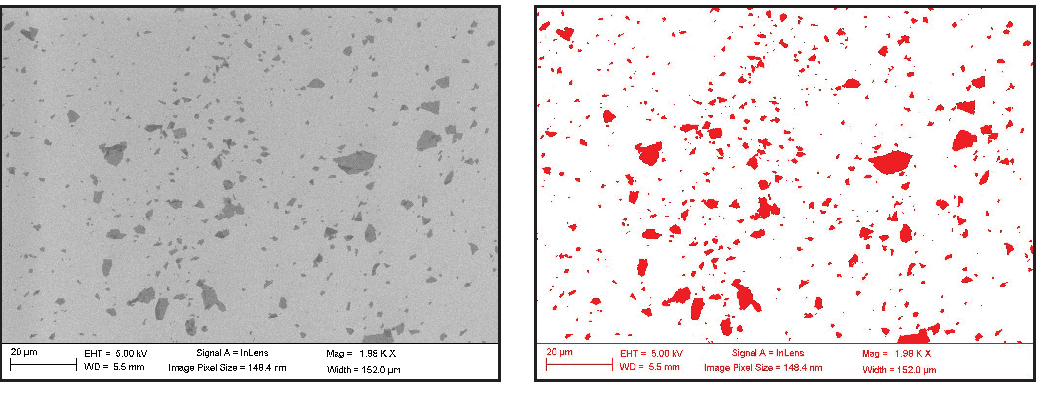
\includegraphics[width=6in]{paper3/FigS1.pdf}
  \caption{\textbf{SEM of monolayer GO and flake size distribution via \textit{ImageJ} analysis.}}
  \label{figS1_AppA}
\end{figure}

Fig.~\ref{figS2_AppA} presents the settling of GO flakes in Sample 1. The photo was taken 10 minute after the injection of GO and highlights the pure colloidal stability of Sample 1.

\begin{figure}[h!]
  \centering
  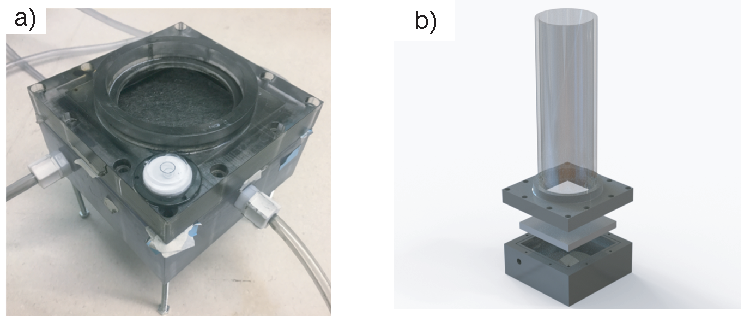
\includegraphics[width=2in]{paper3/FigS2.pdf}
  \caption{\textbf{GO flakes settling.}}
  \label{figS2_AppA}
\end{figure}


Fig.~\ref{figS3_AppA} represents the technique used for determining the GO layer percentage. In the first step, the substrate (silica) is changed to white. Then an intensity histogram is generated followed by deconvolution of the histogram into monolayer and multilayer peaks. The monolayer percentage is then calculated by considering the relative area under each peak in the histogram.

\begin{figure}[t!]
  \centering
  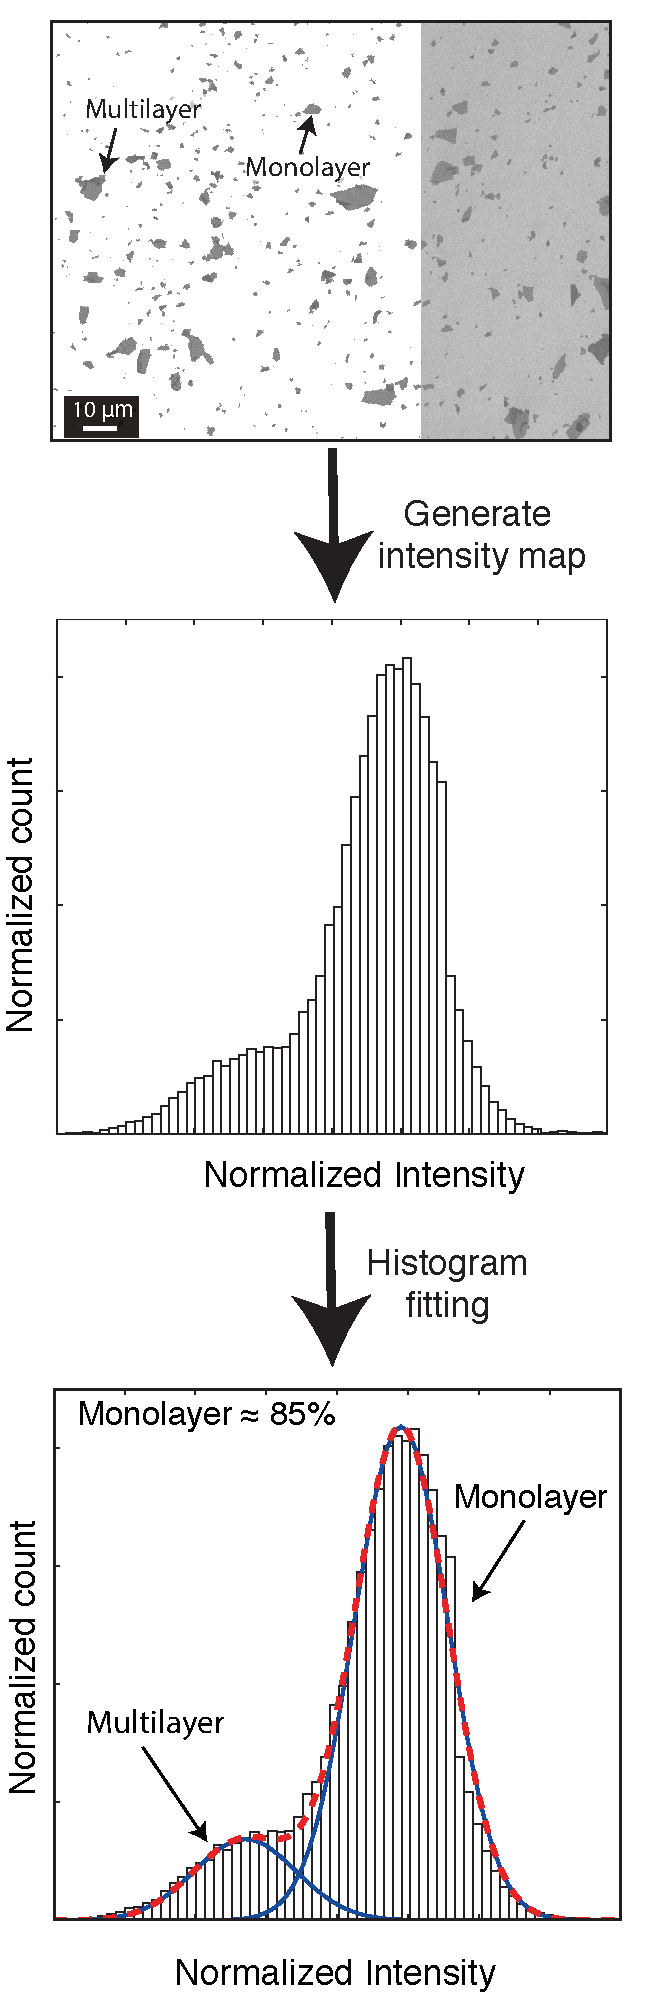
\includegraphics[width=2.8in]{paper3/FigS3.pdf}
  \caption{\textbf{GO monolayer percentage evaluation}}
  \label{figS3_AppA}
\end{figure}

Fig.~\ref{figS4_AppA} collects representative SEM images of bacterial adhesion for Sample 1,2,3,5. Please refer to Figure 7 in the main manuscript for Sample 4 and 6.

\begin{figure}[h!]
  \centering
  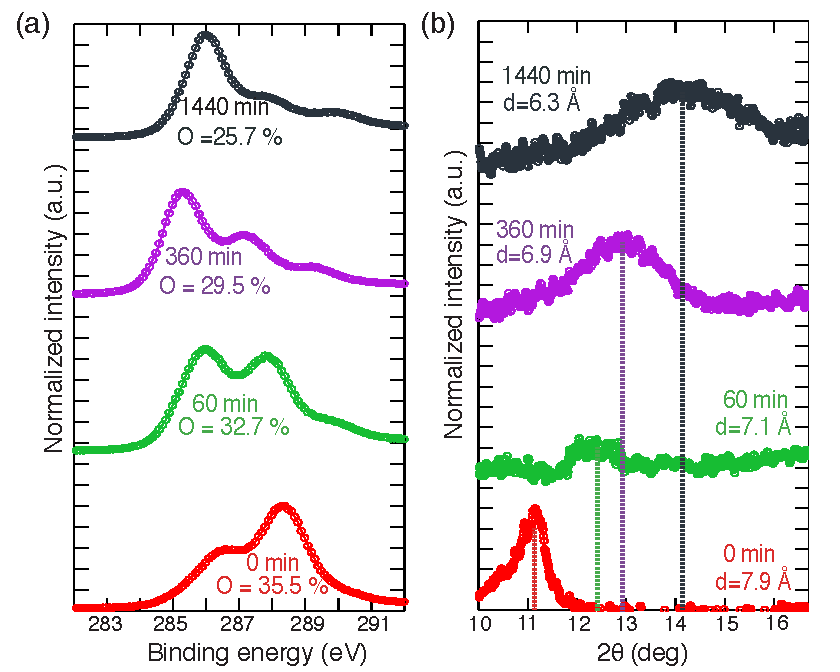
\includegraphics[width=5in]{paper3/FigS4.pdf}
  \caption{\textbf{Representative SEM images of \textit{E. coli} bacteria adhesion onto GOM surfaces.} The samples are identified by numbers.}
  \label{figS4_AppA}
\end{figure}



Fig.~\ref{figS5_AppA} represents the elbow method used to determine the optimal number of clusters used in Fig.~\ref{Fig6_pap3}. Six is the lowest number of clusters to achieve 90\% of variance explained.



\begin{figure}[h!]
  \centering
  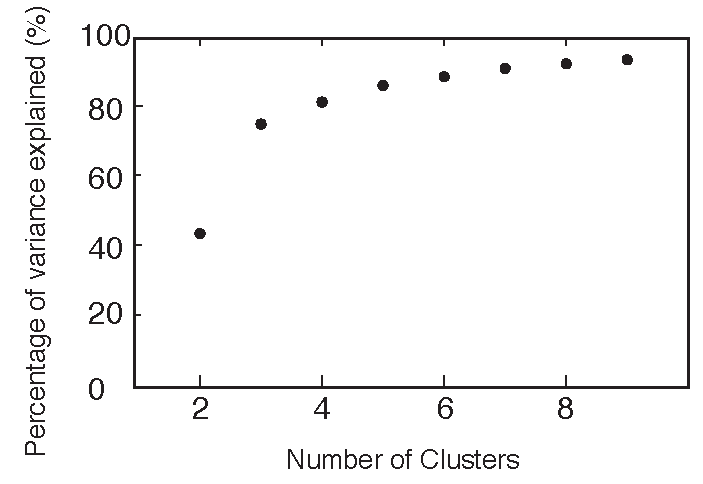
\includegraphics[width=5in]{paper3/FigS5.pdf}
  \caption{\textbf{Elbow method to determine the optimal number of clusters.}}
  \label{figS5_AppA}
\end{figure}



